\subsection{Cliente VPN}

Para se ligar remotamente à rede da sua empresa deverá utilizar um cliente de vpn do tipo PPTP. No caso que a seguir apresentamos a configuração necessária para, a partir de um posto com Windows XP, efectuar uma ligação à empresa.

Para tal deverá seguir os seguintes passos:

Clicar no botão "Iniciar"

Seleccionar "Ligar a..."

Seleccionar "Mostrar todas as ligações"

Seleccionar "Criar uma nova ligação" como ilustra a figura seguinte:

\begin{figure}[H]
    \begin{center}
        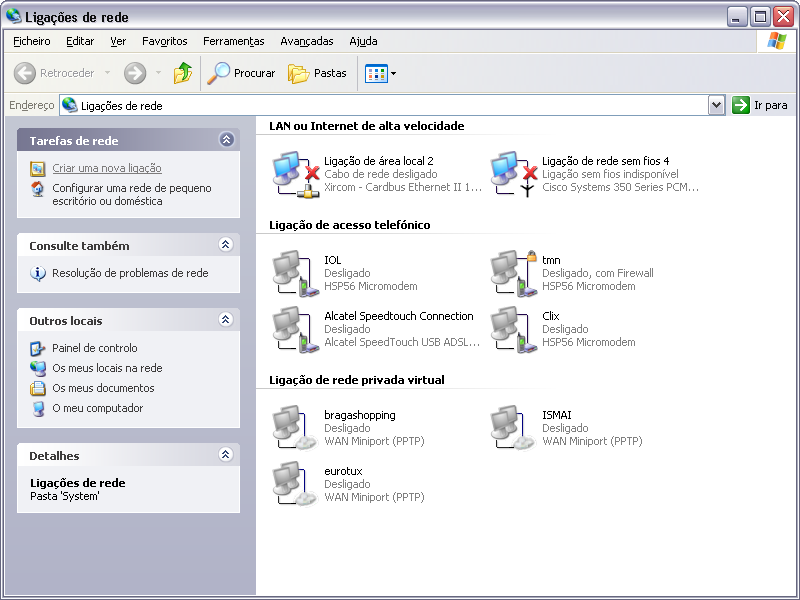
\includegraphics[width=10cm]{include/img/xp_f1}
    \end{center}
    \caption{Ligações de rede}
    \label{fig:XPF1}
\end{figure}

Clique "Seguinte"...

\begin{figure}[H]
    \begin{center}
        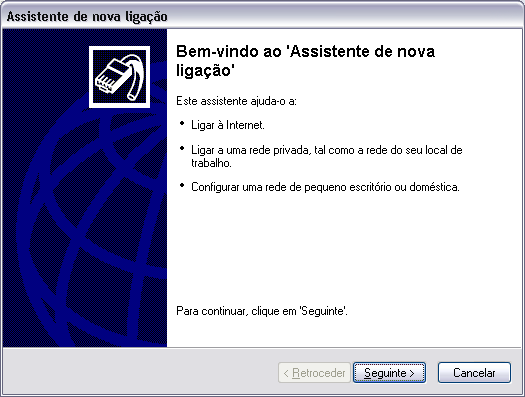
\includegraphics[width=10cm]{include/img/xp_f2}
    \end{center}
    \caption{Assistente de nova ligação}
    \label{fig:XPF2}
\end{figure}

Escolha a opção "Ligar à rede do meu local de trabalho"

\begin{figure}[H]
    \begin{center}
        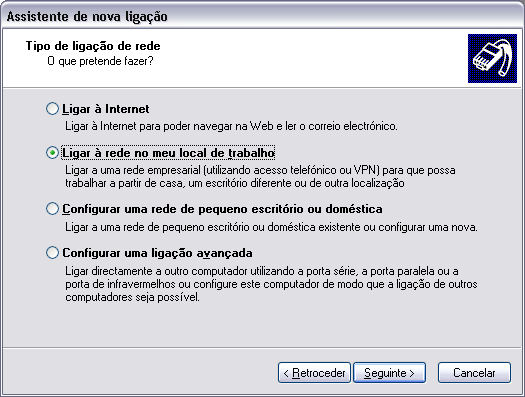
\includegraphics[width=10cm]{include/img/xp_f3}
    \end{center}
    \caption{Tipo de ligação}
    \label{fig:XPF3}
\end{figure}

Escolha a opção "Ligação à rede privada virtual"

\begin{figure}[H]
    \begin{center}
        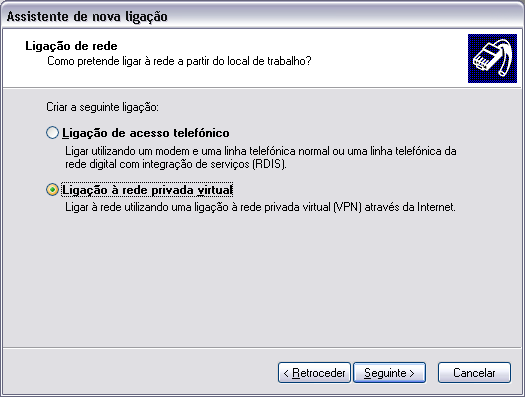
\includegraphics[width=10cm]{include/img/xp_f4}
    \end{center}
    \caption{Ligação VPN}
    \label{fig:XPF4}
\end{figure}

Atribua um nome a esta conexão. Por exemplo "EMPRESA X"

\begin{figure}[H]
    \begin{center}
        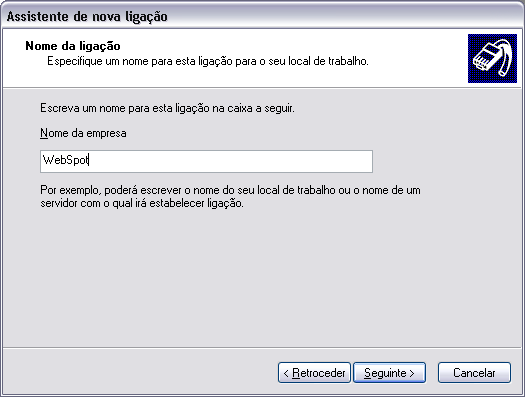
\includegraphics[width=10cm]{include/img/xp_f5}
    \end{center}
    \caption{Nome da ligação}
    \label{fig:XPF5}
\end{figure}

Digite o IP do servidor de  VPN que lhe foi fornecido na documentação.

\begin{figure}[H]
    \begin{center}
        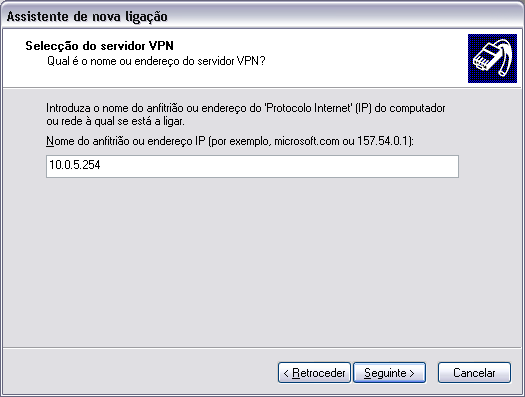
\includegraphics[width=10cm]{include/img/xp_f6}
    \end{center}
    \caption{Selecção do servidor VPN}
    \label{fig:XPF6}
\end{figure}

Seleccione "Criar um atalho ..." se pretende criar um atalho no seu ambiente de trabalho.

\begin{figure}[H]
    \begin{center}
        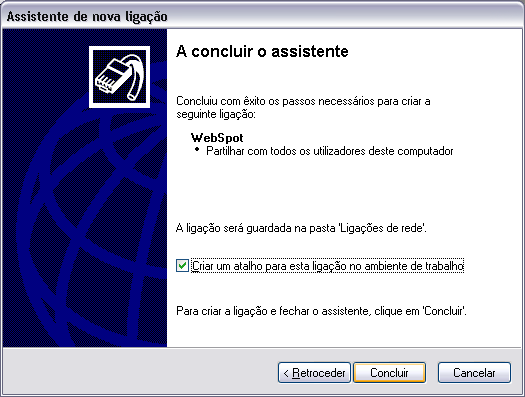
\includegraphics[width=10cm]{include/img/xp_f7}
    \end{center}
    \caption{Criar atalho para a ligação}
    \label{fig:XPF7}
\end{figure}

Digite o par código/senha que lhe foi fornecido

\begin{figure}[H]
    \begin{center}
        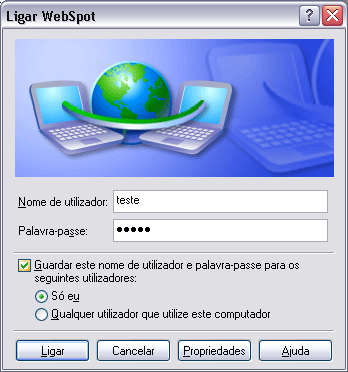
\includegraphics[width=10cm]{include/img/xp_f8}
    \end{center}
    \caption{Ecrã de ligação}
    \label{fig:XPF8}
\end{figure}

Clicar em "Ligar"

\begin{figure}[H]
    \begin{center}
        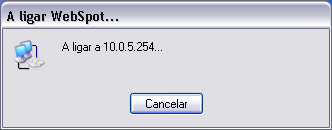
\includegraphics[width=10cm]{include/img/xp_f9}
    \end{center}
    \caption{Estabelecimento da ligação}
    \label{fig:XPF9}
\end{figure}

Após a ligação com sucesso deverá aparecer no canto inferior direito uma informação a indicar o sucesso na ligação.
